\documentclass[aspectratio=169]{beamer}

\usetheme{Madrid}
\usecolortheme{default}
\setbeameroption{hide notes}

\usepackage[T1]{fontenc}
\usepackage[utf8]{inputenc}
\usepackage{lmodern}
\usepackage{booktabs}
\usepackage{tabularx}
\usepackage{tikz}
\usetikzlibrary{positioning,arrows.meta,shapes.geometric}

\definecolor{brand}{RGB}{11,79,108}
\definecolor{accent}{RGB}{0,138,120}
\definecolor{soft}{RGB}{240,247,250}
\setbeamercolor{structure}{fg=brand}
\setbeamercolor{frametitle}{fg=white,bg=brand}
\setbeamercolor{block title}{fg=white,bg=brand}
\setbeamercolor{block body}{bg=soft}
\setbeamertemplate{navigation symbols}{}

\title[Fake News NLP System]{Fake News \& Misinformation Detection System}
\subtitle{End-to-end NLP Seminar Project}
\author{Seminar Project Team}
\institute{HCMUS}
\date{\today}

\begin{document}

\begin{frame}
  \titlepage
\end{frame}

\begin{frame}{Business Problem and Motivation}
  \begin{itemize}
    \item Misinformation spreads faster than manual fact-checking can respond.
    \item Review teams need a fast first-pass triage system with evidence and explanations.
    \item The system is designed as a decision-support tool, not a fully autonomous censor.
  \end{itemize}
  \begin{block}{Success metrics}
    Business: reduce manual triage time and reviewer workload. Technical: accuracy, F1, latency, uncertainty rate, and evidence quality.
  \end{block}
\end{frame}

\begin{frame}{Why NLP and What the System Does}
  \begin{columns}[T,onlytextwidth]
    \column{0.52\textwidth}
    \begin{itemize}
      \item Input is unstructured article text, so semantic understanding is required.
      \item The system combines classification, retrieval, and decision calibration.
      \item Outputs: prediction, confidence, trust score, evidence, and explanation.
    \end{itemize}
    \column{0.40\textwidth}
    \begin{block}{Model stack}
      TF-IDF + Logistic Regression baseline\newline
      RoBERTa main classifier\newline
      Agentic retrieval and decision layer
    \end{block}
  \end{columns}
\end{frame}

\begin{frame}{System Architecture}
\centering
\resizebox{0.95\textwidth}{!}{%
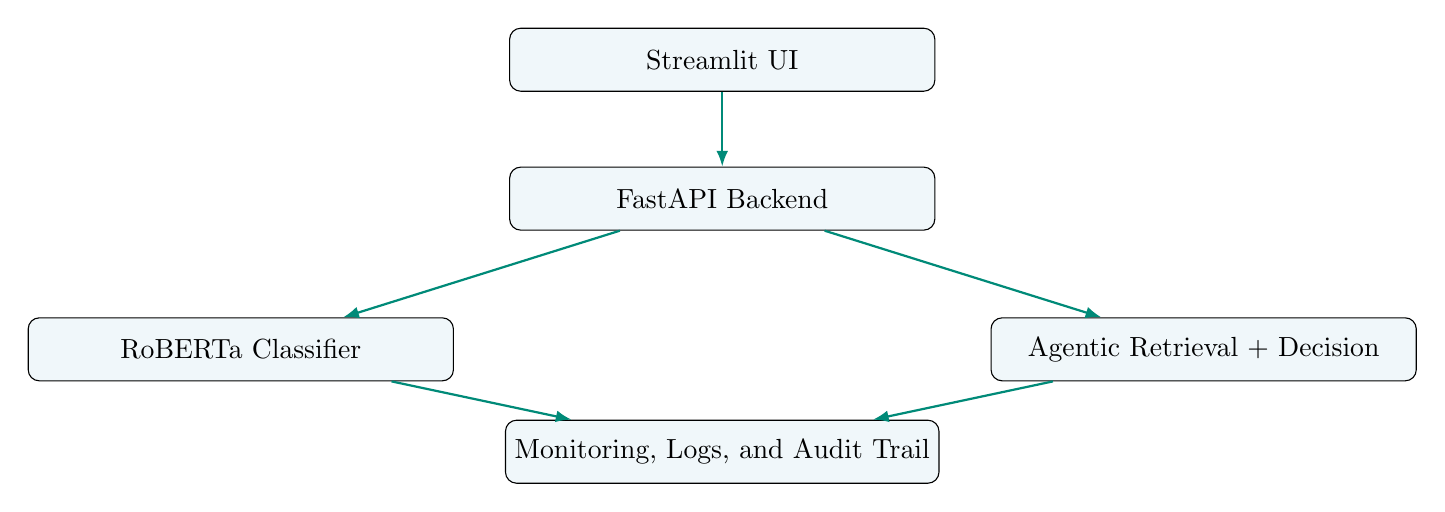
\begin{tikzpicture}[
  node distance=0.95cm,
  block/.style={draw, rounded corners, fill=soft, minimum width=5.4cm, minimum height=0.8cm, align=center},
  arrow/.style={-{Latex[length=2mm]}, thick, draw=accent}
]
\node[block] (ui) {Streamlit UI};
\node[block, below=of ui] (api) {FastAPI Backend};
\node[block, below left=1.1cm and 0.7cm of api] (model) {RoBERTa Classifier};
\node[block, below right=1.1cm and 0.7cm of api] (agent) {Agentic Retrieval + Decision};
\node[block, below=2.4cm of api] (logs) {Monitoring, Logs, and Audit Trail};
\draw[arrow] (ui) -- (api);
\draw[arrow] (api) -- (model);
\draw[arrow] (api) -- (agent);
\draw[arrow] (model) -- (logs);
\draw[arrow] (agent) -- (logs);
\end{tikzpicture}
}
\end{frame}

\begin{frame}{Data Overview}
  \begin{itemize}
    \item English news-style text with binary labels: \texttt{fake} and \texttt{real}.
    \item Split strategy: 70\% train, 15\% validation, 15\% test with stratification.
    \item Cleaning: HTML/URL removal, normalization, duplicate filtering, empty-row handling.
    \item Known risks: source bias, topic imbalance, and out-of-domain generalization gaps.
  \end{itemize}
\end{frame}

\begin{frame}{Model Selection and Evaluation}
  \begin{table}
    \centering
    \small
    \begin{tabular}{lcccc}
      \toprule
      Model & Accuracy & Precision & Recall & F1 \\
      \midrule
      TF-IDF + Logistic Regression & 0.9913 & 0.9938 & 0.9870 & 0.9904 \\
      RoBERTa & 0.9991 & 0.9987 & 0.9997 & 0.9992 \\
      \bottomrule
    \end{tabular}
  \end{table}
  \vspace{0.3em}
  \begin{block}{Trade-off}
    RoBERTa gives the best metrics, while the baseline remains easier to explain and cheaper to run.
  \end{block}
\end{frame}

\begin{frame}{Agentic Workflow}
\centering
\resizebox{0.95\textwidth}{!}{%
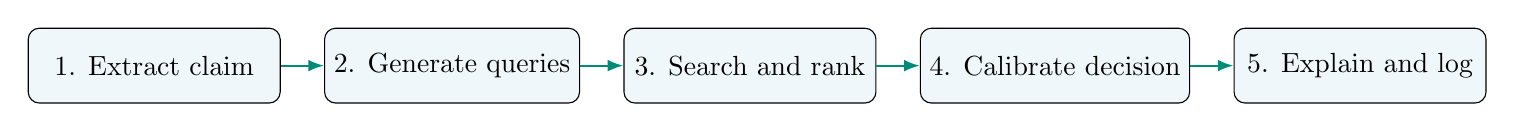
\begin{tikzpicture}[
  node distance=0.55cm and 0.55cm,
  block/.style={draw, rounded corners, fill=soft, minimum width=3.2cm, minimum height=0.95cm, align=center},
  arrow/.style={-{Latex[length=2mm]}, thick, draw=accent}
]
\node[block] (a) {1. Extract claim};
\node[block, right=of a] (b) {2. Generate queries};
\node[block, right=of b] (c) {3. Search and rank};
\node[block, right=of c] (d) {4. Calibrate decision};
\node[block, right=of d] (e) {5. Explain and log};
\draw[arrow] (a) -- (b);
\draw[arrow] (b) -- (c);
\draw[arrow] (c) -- (d);
\draw[arrow] (d) -- (e);
\end{tikzpicture}
}

\vspace{0.35em}
\small Final states: \texttt{REAL}, \texttt{FAKE}, or \texttt{UNCERTAIN} when classifier and evidence disagree.
\end{frame}

\begin{frame}{Recent Hardening and Corrections}
  \begin{itemize}
    \item Claim-centric query generation now prioritizes the assertion over topic words.
    \item Domain-aware fallback was added for science and health claims.
    \item NASA direct search recovers authoritative \texttt{nasa.gov} evidence.
    \item Source credibility now scores subdomains like \texttt{en.m.wikipedia.org} correctly.
    \item Accepted and rejected evidence are logged for debugging and review.
  \end{itemize}
\end{frame}

\begin{frame}{Validation Snapshot}
  \begin{columns}[T,onlytextwidth]
    \column{0.54\textwidth}
    \begin{itemize}
      \item Demo claims now pass the retrieval smoke tests.
      \item Perseverance case now retrieves NASA evidence in live mode.
      \item Trump/Bannon case retrieves Reuters-like evidence and supports reviewable output.
    \end{itemize}
    \column{0.40\textwidth}
    \begin{block}{What this means}
      The retrieval layer is much more reliable for seminar demos, but it still depends on search-provider quality.
    \end{block}
  \end{columns}
\end{frame}

\begin{frame}{Deployment Overview}
  \begin{itemize}
    \item FastAPI backend exposes \texttt{/predict}, \texttt{/analyze}, \texttt{/agent}, \texttt{/health}, and \texttt{/version}.
    \item Streamlit frontend provides a web demo for direct interaction.
    \item Deployment targets: Render for backend and Streamlit Community Cloud for UI.
    \item Monitoring captures latency, confidence drift, uncertainty rate, and conflict rate.
  \end{itemize}
\end{frame}

\begin{frame}{Ethics, Privacy, Robustness}
  \begin{itemize}
    \item Privacy: mask common PII before inference and logging.
    \item Robustness: handle noisy, ambiguous, and out-of-domain claims explicitly.
    \item Ethics: false positives and false negatives can both harm users.
    \item Explainability: evidence, trust score, and rejected-evidence audit trail support human review.
  \end{itemize}
\end{frame}

\begin{frame}{Limitations and Future Work}
  \begin{itemize}
    \item The classifier can still be overconfident on some true claims.
    \item Live retrieval is still sensitive to search noise and snippet quality.
    \item Stronger semantic entailment would improve evidence acceptance.
    \item Future work: better calibration, richer monitoring, and more domain-specific source routing.
  \end{itemize}
  \begin{block}{Why stopping here is acceptable}
    The project already satisfies the seminar deliverables: end-to-end NLP, deployment, agentic behavior, monitoring, and responsible-AI discussion.
  \end{block}
\end{frame}

\begin{frame}{Key Takeaways}
  \begin{itemize}
    \item Built a production-style fake news detection system with retrieval and explainability.
    \item Improved live evidence handling with claim-centric and domain-aware retrieval.
    \item Documented remaining limitations honestly for academic submission.
  \end{itemize}
  \vspace{0.5em}
  \centering
  \Large Q\&A
\end{frame}

\end{document}
